\documentclass[a4paper,10pt]{article}
\usepackage[utf8]{inputenc}
\usepackage[T1]{fontenc}
\usepackage[margin=1in]{geometry}
\usepackage{enumitem}
\usepackage{hyperref}
\usepackage{graphicx}
\usepackage{xcolor}
\usepackage{titlesec}
\usepackage[french]{babel}
\usepackage{helvet}
\renewcommand{\familydefault}{\sfdefault}

\definecolor{sectioncolor}{RGB}{44,62,80}
\definecolor{bubblebg}{RGB}{239,239,239}
\definecolor{bubbletext}{RGB}{51,51,51}

\titleformat{\section}[block]
    {\color{sectioncolor}\normalfont\LARGE\bfseries}
    {}{0ptx}{}

\setlist[itemize,1]{leftmargin=\dimexpr 26pt-.10in, label=\textbullet}

\usepackage{tikz}
\newcommand{\bubble}[1]{%
    \tikz[baseline=(text.base)]{
        \node[draw=none, fill=bubblebg, rounded corners=8pt, inner xsep=6pt, inner ysep=2pt] (text) {\textcolor{bubbletext}{\strut#1}};
    }%
}

\begin{document}

% Header
\begin{center}
    {\LARGE \textbf{Nathan Fitger}}\\[0.5em]
    \textit{Etudiant en master 2 intelligence artificielle à l'universitée de Bordeaux}\\[1em]
        \hspace{0.5em}\href{mailto:nath.fitger@gmail.com}{nath.fitger@gmail.com} \textbar\ 
        \href{https://www.linkedin.com/in/nfitger/}{
\includegraphics[height=1em]{ressources/logo-linkedin.png} Nathan Fitger} \textbar\ 
        \href{https://github.com/0xNatgan}{
\includegraphics[height=1em]{ressources/github.png} 0xNatgan} \textbar\ 
        {
\includegraphics[height=1em]{ressources/appel.png} 07 81 61 31 02}\\
        \href{https://0xNatgan.github.io}{Lien vers mon CV en ligne : 0xNatgan.github.io}
\end{center}

\vspace{1em}

% Photo (top left corner)
\begin{picture}(0,0)
    \put(-20,0){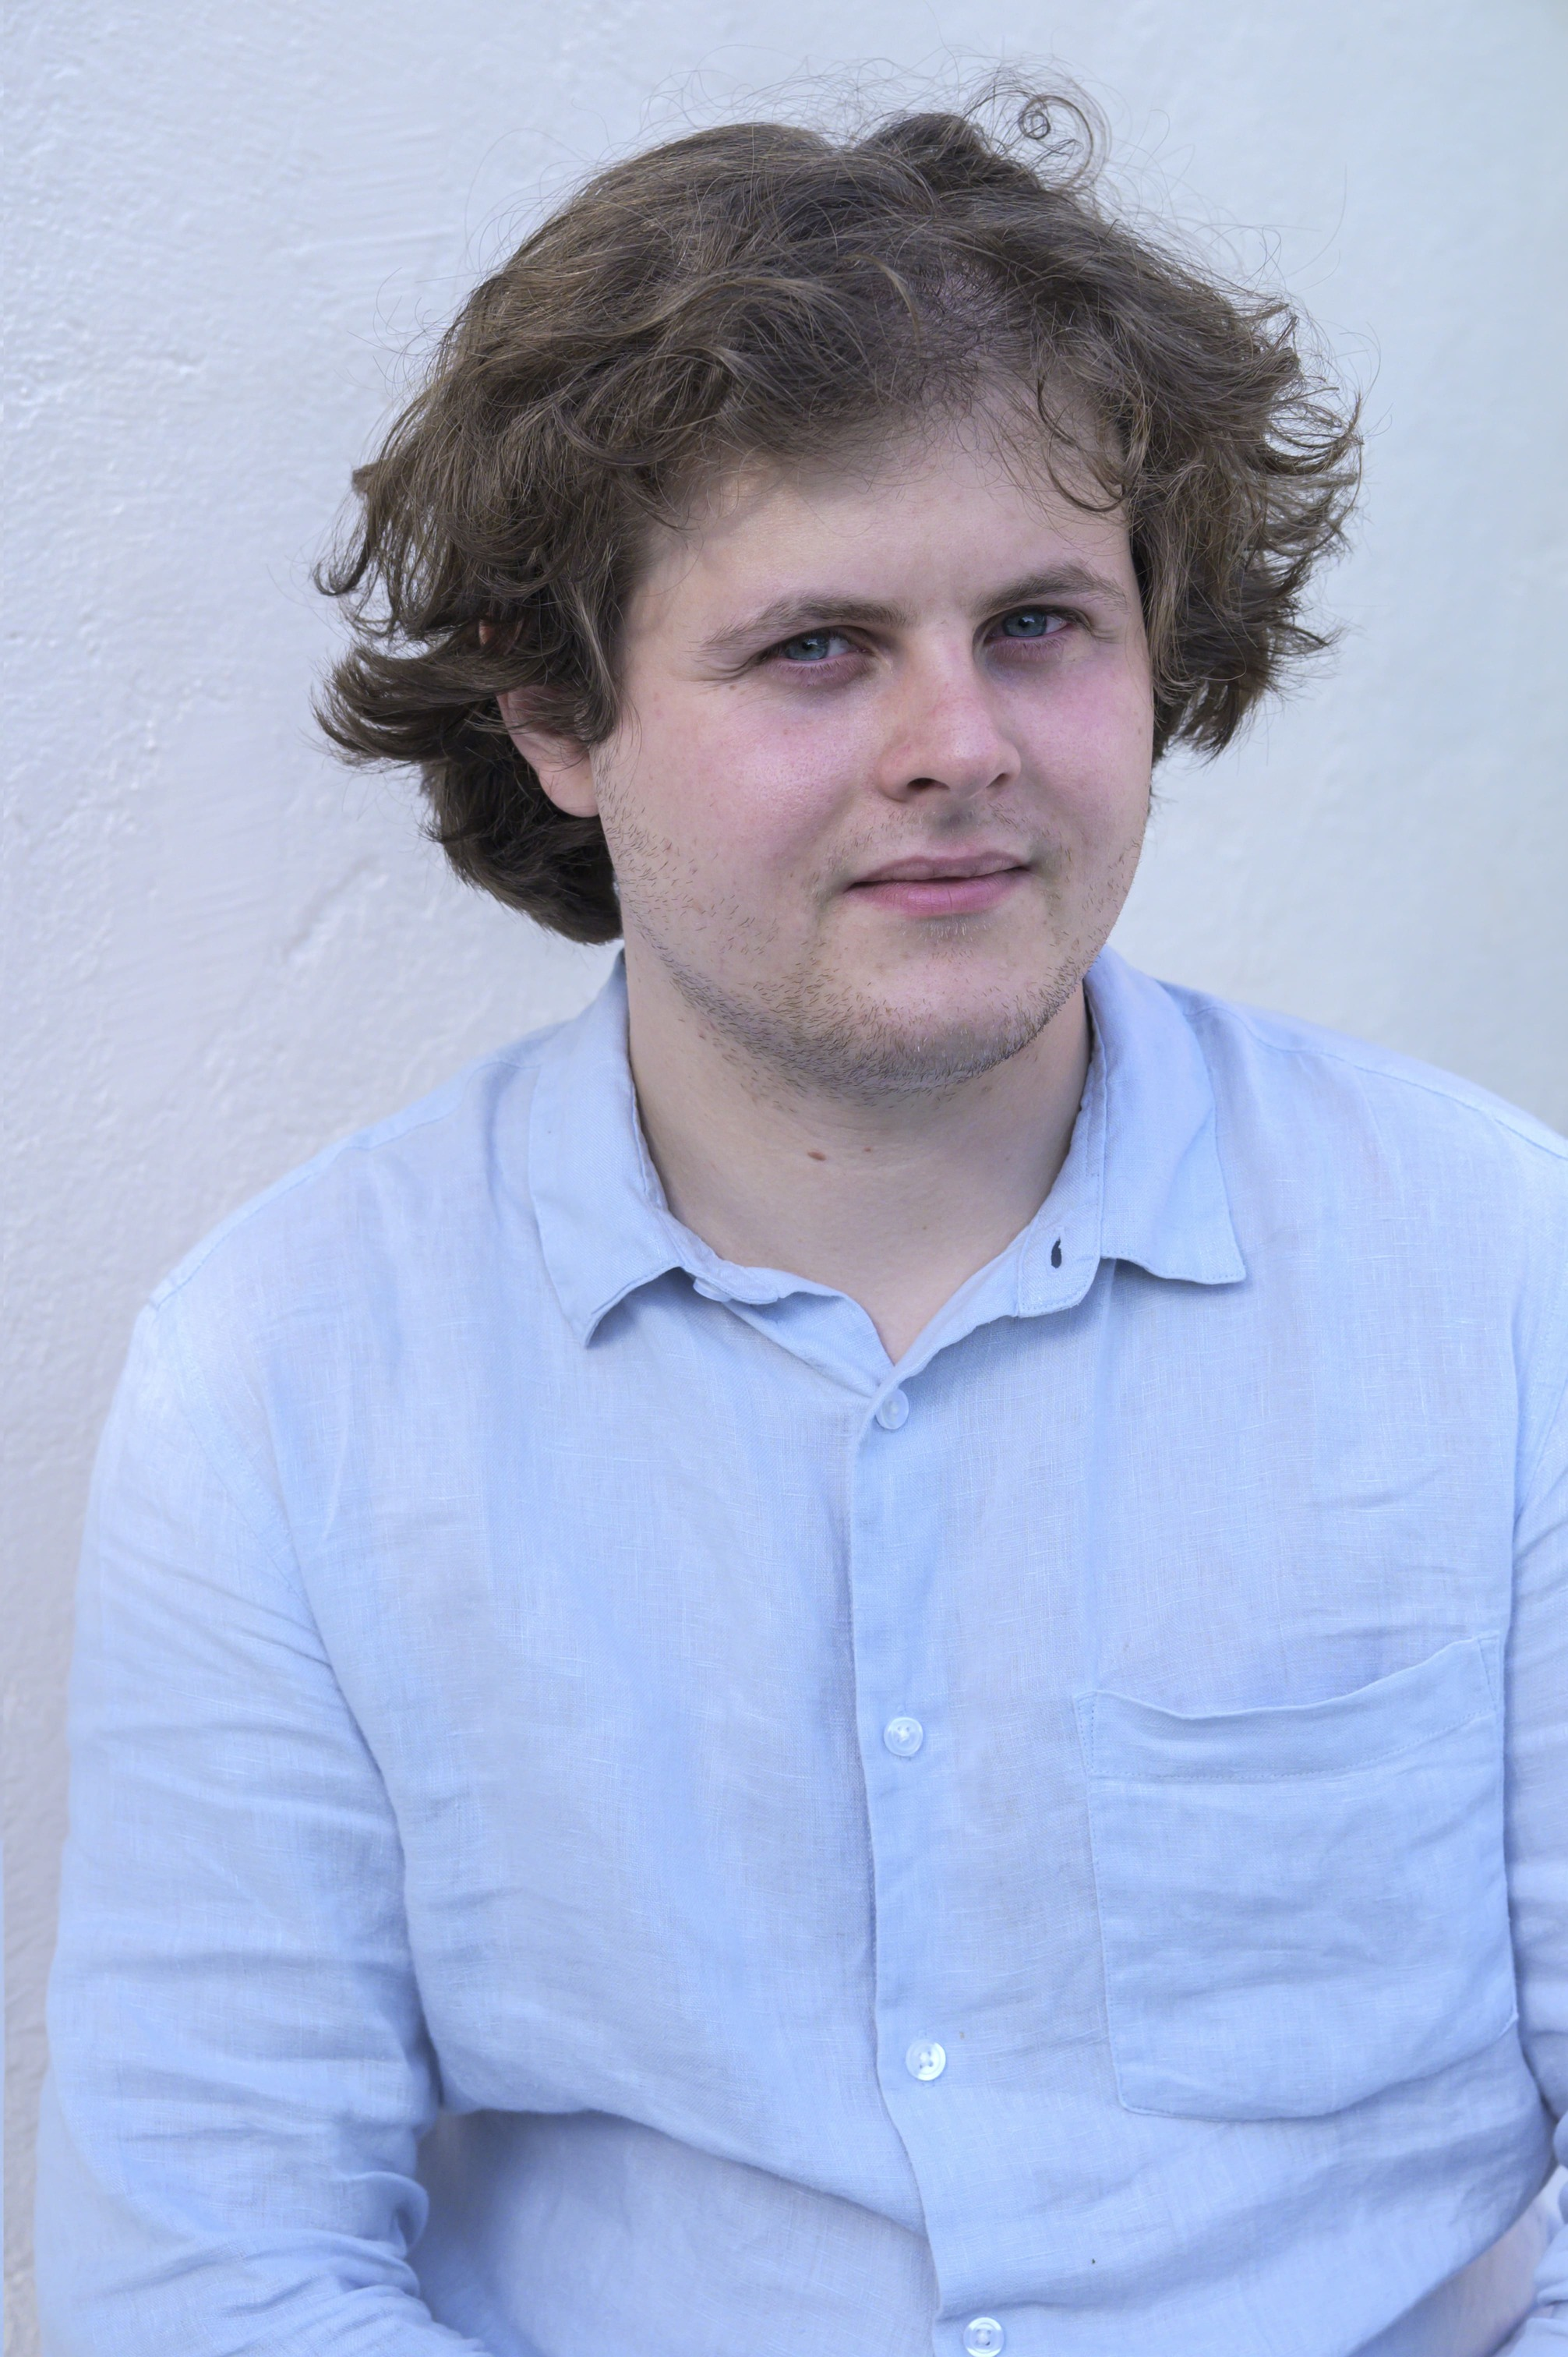
\includegraphics[width=2.2cm]{ressources/photo_cv.jpg}}
\end{picture}

% Profil
\section*{Profil}
Étudiant en intelligence artificielle passionné par l'informatique et les nouvelles technologies, je suis à la recherche d'un stage dans le domaine de l'intelligence artificielle à partir de mars 2026 pour une durée de 6 mois.

Ayant exploré divers domaines tels que la robotique, le web et la cybersécurité avant de me spécialiser en IA, j'ai acquis des compétences solides en programmation et en analyse de données, et je suis toujours à la recherche de nouveaux défis pour élargir mes connaissances.

Au fil de mes expériences en tant que responsable de parc informatique, animateur et concepteur de stages, participant à des CTF et stagiaire en IA, j'ai appris à travailler en équipe et à maîtriser de nouveaux outils et langages de programmation afin de m'adapter aux tâches demandées.
% Compétence
\section*{Compétences}

\noindent \bubble{Python}  \bubble{Scikit-learn} \bubble{Pytorch} \bubble{LSP-servers} \bubble{C} \bubble{C++} \bubble{Java} \bubble{API} \bubble{Machine Learning} \bubble{Deep Learning}  \bubble{Docker} \bubble{Git} \bubble{CTF} \bubble{IA} \bubble{Open source} \bubble{RAG} \bubble{Neural Networks} \bubble{Langage Models} \bubble{SQL} \bubble{HTML} \bubble{CSS} \bubble{GLPI} \bubble{Cybersécurité} \bubble{Robotique} \bubble{Linux} \bubble{Mkdocs} \bubble{Web}  \\
\newline
\noindent\textbf{Langues :} Anglais C1+ (Linguaskill) \textbar\ Allemand B2\\
\noindent\textbf{Mobilité :} Disponible pour des opportunités en France et à l'international

% Expérience
\section*{Expérience}
\noindent\textbf{Stage IA -- Gertrude.fr -- Système de transport intelligent}\\ \hfill \textit{Mai 2025 -- Juillet 2025, Bordeaux}
\begin{itemize}
    \item Création d'un outil de documentation de code utilisant des modèles de langage et du RAG.
    \item Conseil pour l'intégration d'outils d'intelligence artificielle dans l'entreprise.
    \item Participation à des projets de recherche en IA liés au trafic urbain.
\end{itemize}

\noindent\textbf{Responsable du parc informatique, bénévole et trésorier -- Jeunes sciences Bordeaux}\\ \hfill \textit{2019 -- 2025, Bordeaux}
\begin{itemize}
    \item Gestion et maintenance du parc informatique à l'aide de GLPI
    \item Assistance technique aux utilisateurs
    \item Maintenance des équipements informatiques
\end{itemize}

\noindent\textbf{Animateur de stages d'informatique et robotique -- Jeunes sciences Bordeaux}\\ \hfill \textit{2019 -- 2025, Bordeaux}
\begin{itemize}
    \item Conception et animation de stages de robotique et d'informatique pour les jeunes durant les vacances scolaires
\end{itemize}

\noindent\textbf{Jobs d'été en restauration}\\ \hfill \textit{Été 2021 à 2024, Bordeaux}
\begin{itemize}
    \item 2021 : Eklo Bordeaux -- Runner, service en salle, prise de commande et barman
    \item 2023 : Heiko Poké Bègles -- Employé polyvalent de restauration
    \item 2024 : Island Poké -- Employé polyvalent de restauration
\end{itemize}

% Formation
\section*{Formation}
\noindent\textbf{Master Intelligence Artificielle -- Université de Bordeaux} \hfill \textit{2024 -- 2026}\\
\indent Master Intelligence Artificielle. Option Bases de données avancées\\

\noindent\textbf{Licence Informatique -- Université de Bordeaux} \hfill \textit{2020 -- 2024}\\

\noindent\textbf{Formation Développeur Web -- Le Wagon} \hfill \textit{sept. -- nov. 2021}\\
\indent Formation intensive au développement web\\

\noindent\textbf{Baccalauréat Scientifique -- Lycée Vaclav Havel} \hfill \textit{2019--2020}\\


% Projets
\section*{Projets}
\noindent\textbf{DocGen\_LLM} (\href{https://github.com/0xNatgan/DocGen_LLM}{github.com/0xNatgan/DocGen\_LLM})\\
Outil de génération de documentation de code à l'aide de modèles de langage et de RAG.\\

\noindent
\bubble{Python} \bubble{Docker} \bubble{Serveurs de langage} \bubble{LLM} \bubble{RAG} \bubble{documentation} \bubble{mkdocs} \bubble{Markdown} \bubble{HTML} \bubble{open source} \bubble{IA}\\

\begin{itemize}
    \item Problématique principale : Générer une documentation de code de manière automatisée et agnostique au langage dans le cadre de projets manquant de documentation et/ou ayant une documentation peu claire.
    \item DocGen\_LLM est un outil de génération de documentation de code qui utilise des modèles de langage en combinaison avec des serveurs de langage pour générer une documentation claire et concise pour l'ensemble d'une base de code. Il est conçu pour être indépendant du langage de programmation. L'outil s'intègre facilement avec des outils de lecture de documentation comme mkdocs. Il permet de générer une documentation à ajouter au code ou à utiliser dans une documentation externe au format Markdown ou HTML.
\end{itemize}
\noindent\textbf{Serveur de langage TCL} (\href{https://github.com/0xNatgan/tcl-lsp}{github.com/0xNatgan/tcl-lsp})\\
Serveur de langage TCL pour l'analyse de code.\\

\noindent
\bubble{TCL} \bubble{Serveur de langage} \bubble{TCP} \bubble{stdin/out}\\

\begin{itemize}
    \item Problématique principale : Dans le cadre d'un besoin d'analyse d'un projet en TCL, j'ai développé un serveur de langage pour faciliter cette tâche et la rendre possible avec mon projet DocGen\_LLM.
    \item Ce serveur de langage permet d'analyser le code TCL et d'en extraire des informations selon le standard LSP. Ce projet est une implémentation simple d'un serveur de langage TCL avec les capacités suivantes : extraction de symboles, recherche de définitions ainsi que de références. Ce projet comprend une interface stdin/out et TCP.
\end{itemize}

\noindent\textbf{Quoridor}

Jeu de société Quoridor développé en Java avec une interface graphique et des IA. Projet réalisé dans le cadre des cours de l'Université de Bordeaux.\\

\noindent
\bubble{Java} \bubble{IA} \bubble{Graphique} \bubble{JavaFx} \bubble{Junit}\\

\begin{itemize}
    \item Problématique principale : Développer un jeu de société Quoridor en Java avec une interface graphique et des IA pour jouer contre l'utilisateur.
    \item Ce projet comprend une implémentation du jeu Quoridor avec une interface graphique en Java et des IA pour jouer contre l'utilisateur ainsi que des statistiques avancées sur les algorithmes d'IA utilisés.
\end{itemize}

\end{document}